\documentclass{article}
\usepackage[utf8]{inputenc}
\usepackage{mathtools}
\usepackage{amsmath}
\usepackage{amsfonts} 
\usepackage{tikz}
\usetikzlibrary{positioning}
\usepackage{graphicx}
\graphicspath{ {./images/} }
\setlength{\parindent}{0pt}

\title{Physics Informed Neural Networks. \\A complete explanation for beginners}
\author{Christian Ortiz}

\begin{document}

\maketitle

\begin{abstract}
In this tutorial we first discuss a simple toy model that describes a time-dependent one dimensional system. This toy model allows the reader to not only understand how physics informed neural networks are implemented but also to understand how the \textit{autograd} and the \textit{backpropagation} functions work. In particular, how the former handles second order derivatives and how the latter may be given considering a forward gradient descent. We then extend this model to consider a time-dependent three dimensional system in a deep learning architecture, and explore novel computational approaches.
\end{abstract}

\section{Introduction}
Partial derivatives are core ingredients in neural network architectures. However, they have been mostly overlooked... blah blah.



\section{Toy Model}
To have a solid understanding of physics informed neural networks, we first construct a simple toy model developing our own \textit{autograd} and \textit{backpropagation} functions. We start discussing these functions from a mathematical perspective and then we implement our physics informed architecture. In the following section, which handles a general model, we consider a similar approach, but from a computational perspective. In this sense, here we do not explicitly address the difference between the \textit{forward} and \textit{reverse} modes or the JVP and VJP approaches, instead we just give a general introduction. 

\newpage
\subsection{System} 

The following neural network is considered: 
\tikzset{%
  every neuron/.style={
    circle,
    draw,
    minimum size=1cm
  },
  neuron missing/.style={
    draw=none, 
    scale=4,
    text height=0.333cm,
    execute at begin node=\color{black}$\vdots$
  },
}

\begin{figure}[ht]
\centering
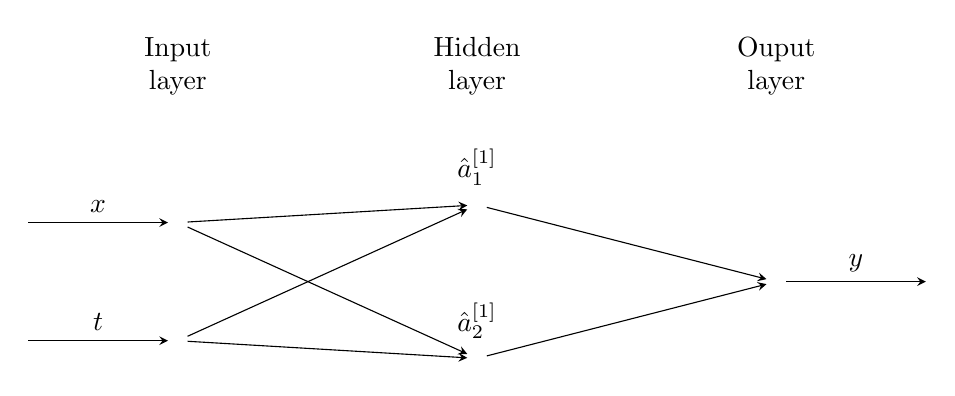
\begin{tikzpicture}[x=1.9cm, y=1.5cm, >=stealth]

\foreach \m [count=\y] in {1,2}
  \node [every neuron/.try, neuron \m/.try] (input-\m) at (4.5,1-\y) {};

\foreach \m [count=\y] in {1}
  \node [every neuron/.try, neuron \m/.try ] (hidden-\m) at (6.5,-0.15-\y) {};
\foreach \m [count=\y] in {2}
  \node [every neuron/.try, neuron \m/.try ] (hidden-\m) at (6.5,1.15-\y) {};

\foreach \m [count=\y] in {1}
  \node [every neuron/.try, neuron \m/.try ] (output-\m) at (8.5,0.5-\y) {};
  
  

\foreach \l [count=\i] in {x,t}
  \draw [<-] (input-\i) -- ++(-1,0)
    node [above, midway] {$\l$};

\foreach \l [count=\i] in {2,1}
  \node [above] at (hidden-\i.north) {$\hat a_{\l}^{[1]}$};

\foreach \l [count=\i] in {1}
  \draw [->] (output-\i) -- ++(1,0)
    node [above, midway] {$y$};
    
    

\foreach \i in {1,2}
  \foreach \j in {1,2}
    \draw [->] (input-\i) -- (hidden-\j);
    
\foreach \i in {1,2}
  \foreach \j in {1}
    \draw [->] (hidden-\i) -- (output-\j);
    
    

\foreach \l [count=\x from 1] in {Input, Hidden, Ouput}
  \node [align=center, above] at (\x*2.0+2.5,1) {\l \\ layer};
\end{tikzpicture}
\caption{A neural network with 2 input parameters ($x,t$), 1 hidden layer with 2 neurons, and 1 output ($y$).}
\end{figure}

For simplicity, we set the following:

\begin{align}
\label{eq:x}
x = a_1^{[0]},\\
t = a_2^{[0]},\\
y = a_1^{[2]}.
\end{align}

Then we have,

\begin{align}
\label{eq:a1-1}
a_1^{[1]} = g_1\left(z_1^{[1]}\right) = g_1\left(w_{11}^{[1]} a_1^{[0]} + w_{12}^{[1]} a_2^{[0]} + b_1^{[1]}\right), \\
\label{eq:a2-1}
a_2^{[1]} = g_1\left (z_2^{[1]} \right) = g_1\left(w_{21}^{[1]} a_1^{[0]} + w_{22}^{[1]} a_2^{[0]} + b_2^{[1]}\right), \\
\label{eq:a1-2}
a_1^{[2]} = g_2\left (z_1^{[2]} \right) = g_2\left(w_{11}^{[2]} a_1^{[1]} + w_{12}^{[2]} a_2^{[1]} + b_1^{[2]}\right).
\end{align}

$a_i^{[k]}=g_{k}(z_i^{[k]})$ is the activation function. $w_{ij}^{[k]}$ is the weight, and $b_i^{[k]}$ is the bias. $k$ denotes the layer index and $i$ ($j$) denotes the row (column) of the matrix.
In vectorial form the above expressions read,
\begin{align}
\textbf{a}^{[0]} = 
\begin{pmatrix}
a_1^{[0]} \\
a_2^{[0]}
\end{pmatrix}, ~~
\textbf{a}^{[1]} &= 
\begin{pmatrix}
a_1^{[1]} \\
a_2^{[1]}
\end{pmatrix}, ~~~~~~~~~~~~
a^{[2]} = 
a_1^{[2]}, \\
\textbf{z}^{[1]} &= 
\begin{pmatrix}
z_1^{[1]} \\
z_2^{[1]}
\end{pmatrix}, ~~~~~~~~~~~~
z^{[2]} = 
z_1^{[2]}, \\
\textbf{b}^{[1]} &= 
\begin{pmatrix}
b_{1}^{[1]} \\ b_{2}^{[1]}
\end{pmatrix}, ~~~~~~~~~~~~
b^{[2]} = 
b_{1}^{[2]}, \\
\textbf{w}^{[1]} &= 
\begin{pmatrix}
w_{11}^{[1]} & w_{12}^{[1]}    \\
w_{21}^{[1]} & w_{22}^{[1]}
\end{pmatrix}, ~~
\textbf{w}^{[2]} = 
\begin{pmatrix}
w_{11}^{[2]} & w_{12}^{[2]}
\end{pmatrix},
\end{align}

where we have,
\begin{align}
\label{eq:vector-a1}
\textbf{a}^{[1]} &= g_1(\textbf{z}^{[1]}) = g_1\left(\textbf{w}^{[1]}\cdot \textbf{a}^{[0]} + \textbf{b}^{[1]}\right),\\
y = a^{[2]} &= g_2(z^{[2]}) = g_2\left(\textbf{w}^{[2]}\cdot \textbf{a}^{[1]} + b^{[2]}\right). 
\label{eq:vector-a2}
\end{align}

Eq. \eqref{eq:vector-a1} is equivalent to Eqs. \eqref{eq:a1-1}-\eqref{eq:a2-1} and Eq. \eqref{eq:vector-a2} is equivalent to Eq. \eqref{eq:a1-2}.

\subsection{Autograd}
Considering Eqs. \eqref{eq:x}-\eqref{eq:a1-2} we have,
\begin{align}
\label{eq:long}
y = g_2\Bigg{(}w_{11}^{[2]} g_1\left(w_{11}^{[1]} x + w_{12}^{[1]} t + b_1^{[1]}\right) +
             w_{12}^{[2]} g_1\left(w_{21}^{[1]} x + w_{22}^{[1]} t + b_2^{[1]}\right) + b_1^{[2]}\Bigg{)}.
\end{align}
If we want to compute $\frac{\partial y}{\partial x}$ and $\frac{\partial y}{\partial t}$, in Eq. \eqref{eq:long} it is enough to derive with respect to $x$ and $t$; however, this procedure is extensive. A better approach in multivariate calculus is to consider the Jacobian matrix. To do so, first, the chain rule differentiation gives us:

\begin{align}
\label{dyda0}
\frac{\partial y}{\partial \textbf{a}^{[0]}} = \frac{\partial y}{\partial z^{[2]}} \frac{\partial z^{[2]}}{\partial \textbf{a}^{[1]}} \frac{\partial \textbf{a}^{[1]}}{\partial \textbf{z}^{[1]}}  \frac{\partial \textbf{z}^{[1]}}{\partial \textbf{a}^{[0]}}. 
\end{align}

Each term is given by,

\begin{align}
\frac{\partial y}{\partial z^{[2]}} &= g_2'(z^{[2]}),\\
\frac{\partial z^{[2]}}{\partial \textbf{a}^{[1]}} &=
\begin{pmatrix}
\frac{\partial z^{[2]}}{\partial a_1^{[1]}} & \frac{\partial z^{[2]}}{\partial a_2^{[1]}}
\end{pmatrix}, \\
\frac{\partial \textbf{a}^{[1]}}{\partial \textbf{z}^{[1]}} &=
\begin{pmatrix}
\frac{\partial a_1^{[1]}}{\partial z_1^{[1]}} & \frac{\partial a_1^{[1]}}{\partial z_2^{[1]}} \\
\frac{\partial a_2^{[1]}}{\partial z_1^{[1]}} & \frac{\partial a_2^{[1]}}{\partial z_2^{[1]}}
\end{pmatrix}, \\
\frac{\partial \textbf{z}^{[1]}}{\partial \textbf{a}^{[0]}} &=
\begin{pmatrix}
\frac{\partial z_1^{[1]}}{\partial x} & 
\frac{\partial z_1^{[1]}}{\partial t} \\
\frac{\partial z_2^{[1]}}{\partial x} &
\frac{\partial z_2^{[1]}}{\partial t}
\end{pmatrix}.
\end{align}

In the above expressions, the matrices are the so called Jacobian matrices. The dimension of each Jacobian matrix is $n \times m$, where $n$ ($m$) refers to the dimension of the numerator (denominator) in the partial derivative. To solve these expressions we consider Eqs. \eqref{eq:a1-1}-\eqref{eq:a1-2}; therefore, we have,

\begin{align}
\label{comp1}
\frac{\partial y}{\partial z^{[2]}} &= g_2'(z^{[2]}),\\
\frac{\partial z^{[2]}}{\partial \textbf{a}^{[1]}} &=
\begin{pmatrix}
w_{11}^{[2]} & w_{12}^{[2]} 
\end{pmatrix}, \\
\frac{\partial \textbf{a}^{[1]}}{\partial \textbf{z}^{[1]}} &=
\begin{pmatrix}
g_1'(z_1^{[1]}) & 0 \\
0 & g_1'(z_2^{[1]})
\end{pmatrix}, \\
\frac{\partial \textbf{z}^{[1]}}{\partial \textbf{a}^{[0]}} &=
\begin{pmatrix}
w_{11}^{[1]} & w_{12}^{[1]} \\
w_{21}^{[1]} & w_{22}^{[1]}
\end{pmatrix}.
\label{comp4}
\end{align}

Consequently, $\frac{\partial y}{\partial \textbf{a}^{[0]}}$ reads,

\begin{align}
\frac{\partial y}{\partial \textbf{a}^{[0]}} &= g_2'(z^{[2]})
\begin{pmatrix}
w_{11}^{[2]} & w_{12}^{[2]} 
\end{pmatrix}
\begin{pmatrix}
g_1'(z_1^{[1]}) & 0 \\
0 & g_1'(z_2^{[1]})
\end{pmatrix}
\begin{pmatrix}
w_{11}^{[1]} & w_{12}^{[1]} \\
w_{21}^{[1]} & w_{22}^{[1]}
\end{pmatrix}. 
\end{align}

To solve for each component we consider directional unit vectors of the form $\textbf{e}_x = \begin{pmatrix}
1 \\
0
\end{pmatrix}$ and $\textbf{e}_t =  \begin{pmatrix}
0 \\
1
\end{pmatrix}$, then we have, 

\begin{align}
\frac{\partial y}{\partial x}  &= \frac{\partial y}{\partial \textbf{a}^{[0]}} \cdot \textbf{e}_x,   \\
\frac{\partial y}{\partial t} &= \frac{\partial y}{\partial \textbf{a}^{[0]}} \cdot \textbf{e}_t,
\end{align}

which gives us,


\begin{align}
\frac{\partial y}{\partial x} &= g_2'(z^{[2]})
\begin{pmatrix}
w_{11}^{[2]} & w_{12}^{[2]} 
\end{pmatrix}
\begin{pmatrix}
g_1'(z_1^{[1]}) & 0 \\
0 & g_1'(z_2^{[1]})
\end{pmatrix}
\begin{pmatrix}
w_{11}^{[1]} & w_{12}^{[1]} \\
w_{21}^{[1]} & w_{22}^{[1]}
\end{pmatrix}
\begin{pmatrix}
1 \\
0
\end{pmatrix}  \\
&= g_2'(z^{[2]})
\begin{pmatrix}
w_{11}^{[2]} & w_{12}^{[2]} 
\end{pmatrix}
\begin{pmatrix}
g_1'(z_1^{[1]}) & 0 \\
0 & g_1'(z_2^{[1]})
\end{pmatrix}
\begin{pmatrix}
w_{11}^{[1]}  \\
w_{21}^{[1]}
\end{pmatrix} \\
&= g_2'(z^{[2]})
\begin{pmatrix}
w_{11}^{[2]} & w_{12}^{[2]} 
\end{pmatrix}
\begin{pmatrix}
g_1'(z_1^{[1]}) w_{11}^{[1]} \\
g_1'(z_2^{[1]}) w_{21}^{[1]}
\end{pmatrix} \\
&= g_2'\left(z_1^{[2]}\right)\Bigg{(} w_{11}^{[2]} g_1'(z_1^{[1]})w_{11}^{[1]} + w_{12}^{[2]}g_1'(z_2^{[1]})w_{21}^{[1]} \Bigg{)}.
\end{align}

and

\begin{align}
\frac{\partial y}{\partial t} &= g_2'(z^{[2]})
\begin{pmatrix}
w_{11}^{[2]} & w_{12}^{[2]} 
\end{pmatrix}
\begin{pmatrix}
g_1'(z_1^{[1]}) & 0 \\
0 & g_1'(z_2^{[1]})
\end{pmatrix}
\begin{pmatrix}
w_{11}^{[1]} & w_{12}^{[1]} \\
w_{21}^{[1]} & w_{22}^{[1]}
\end{pmatrix}
\begin{pmatrix}
0 \\
1
\end{pmatrix} \\
&= g_2'(z^{[2]})
\begin{pmatrix}
w_{11}^{[2]} & w_{12}^{[2]} 
\end{pmatrix}
\begin{pmatrix}
g_1'(z_1^{[1]}) & 0 \\
0 & g_1'(z_2^{[1]})
\end{pmatrix}
\begin{pmatrix}
w_{12}^{[1]}  \\
w_{22}^{[1]}
\end{pmatrix}\\
&= g_2'(z^{[2]})
\begin{pmatrix}
w_{11}^{[2]} & w_{12}^{[2]} 
\end{pmatrix}
\begin{pmatrix}
g_1'(z_1^{[1]}) w_{12}^{[1]} \\
g_1'(z_2^{[1]}) w_{22}^{[1]}
\end{pmatrix} \\
&= g_2'\left(z_1^{[2]}\right)\Bigg{(} w_{11}^{[2]} g_1'(z_1^{[1]})w_{12}^{[1]} + w_{12}^{[2]}g_1'(z_2^{[1]})w_{22}^{[1]} \Bigg{)}.
\end{align}

As you can see, in the above expressions we have multiplied the Jacobian matrices from right to left, this is called the \textit{forward} mode, an approach to be discussed in more detail when studying the general model. Now let's consider the second derivative. We previously had,

\begin{align}
\label{dydxgeneral}
\frac{\partial y}{\partial \textbf{a}^{[0]}} = 
\begin{pmatrix}
\frac{\partial y}{\partial x}  &
\frac{\partial y}{\partial t} 
\end{pmatrix}. 
\end{align}

The second derivative reads,

\begin{align}
\label{d2ydx2general}
\left(\frac{\partial}{\partial \textbf{a}^{[0]}}\right)^T \cdot \left(\frac{\partial y}{\partial \textbf{a}^{[0]}}\right)  &= \begin{pmatrix}
\frac{\partial }{\partial x}  \\
\frac{\partial }{\partial t} 
\end{pmatrix} \cdot\begin{pmatrix}
\frac{\partial y}{\partial x}  &
\frac{\partial y}{\partial t} 
\end{pmatrix} = 
\begin{pmatrix}
\frac{\partial^2 y}{\partial x^2}  & \frac{\partial^2 y}{\partial x \partial t} \\
\frac{\partial^2 y}{\partial t \partial x} & \frac{\partial^2 y}{\partial t^2} \\
\end{pmatrix}.
\end{align}

Replacing Eq. \eqref{dyda0} in Eq. \eqref{d2ydx2general} we have,

\begin{align}
\left(\frac{\partial}{\partial \textbf{a}^{[0]}}\right)^T \cdot \left(\frac{\partial y}{\partial \textbf{a}^{[0]}}\right)  
&= \left(\frac{\partial}{\partial \textbf{a}^{[0]}}\right)^T \cdot \left( \frac{\partial y}{\partial z^{[2]}} \frac{\partial z^{[2]}}{\partial \textbf{a}^{[1]}} \frac{\partial \textbf{a}^{[1]}}{\partial \textbf{z}^{[1]}}  \frac{\partial \textbf{z}^{[1]}}{\partial \textbf{a}^{[0]}}\right) \\
&= 
\begin{pmatrix}
\frac{\partial }{\partial x}  \\
\frac{\partial }{\partial t} 
\end{pmatrix}  \cdot 
\begin{pmatrix}
 \frac{\partial y}{\partial z^{[2]}} \frac{\partial z^{[2]}}{\partial \textbf{a}^{[1]}} \frac{\partial \textbf{a}^{[1]}}{\partial \textbf{z}^{[1]}}  \frac{\partial \textbf{z}^{[1]}}{\partial x}  &
 \frac{\partial y}{\partial z^{[2]}} \frac{\partial z^{[2]}}{\partial \textbf{a}^{[1]}} \frac{\partial \textbf{a}^{[1]}}{\partial \textbf{z}^{[1]}}  \frac{\partial \textbf{z}^{[1]}}{\partial t} 
\end{pmatrix} \\
&= 
\begin{pmatrix}
\frac{\partial }{\partial x}\left( \frac{\partial y}{\partial z^{[2]}} \frac{\partial z^{[2]}}{\partial \textbf{a}^{[1]}} \frac{\partial \textbf{a}^{[1]}}{\partial \textbf{z}^{[1]}}  \frac{\partial \textbf{z}^{[1]}}{\partial x}\right) &
\frac{\partial }{\partial x}\left(\frac{\partial y}{\partial z^{[2]}} \frac{\partial z^{[2]}}{\partial \textbf{a}^{[1]}} \frac{\partial \textbf{a}^{[1]}}{\partial \textbf{z}^{[1]}}  \frac{\partial \textbf{z}^{[1]}}{\partial t}\right)
\\
\frac{\partial }{\partial t} \left(\frac{\partial y}{\partial z^{[2]}} \frac{\partial z^{[2]}}{\partial \textbf{a}^{[1]}} \frac{\partial \textbf{a}^{[1]}}{\partial \textbf{z}^{[1]}}  \frac{\partial \textbf{z}^{[1]}}{\partial x}\right)
&
\frac{\partial }{\partial t} \left(\frac{\partial y}{\partial z^{[2]}} \frac{\partial z^{[2]}}{\partial \textbf{a}^{[1]}} \frac{\partial \textbf{a}^{[1]}}{\partial \textbf{z}^{[1]}}  \frac{\partial \textbf{z}^{[1]}}{\partial t}\right)
\end{pmatrix}.  
\end{align}


In the above expression, only the terms that depend on $z$, intrinsically depend on $x$ and $t$. As an example let's consider $\frac{\partial^2 y}{\partial x^2}$, then we have: 


\begin{align}
\frac{\partial^2 y}{\partial x^2}
&=\frac{\partial}{\partial x}\left( \frac{\partial y}{\partial z^{[2]}} \frac{\partial z^{[2]}}{\partial \textbf{a}^{[1]}} \frac{\partial \textbf{a}^{[1]}}{\partial \textbf{z}^{[1]}}  \frac{\partial \textbf{z}^{[1]}}{\partial x}\right) \\
&= \left( \frac{\partial}{\partial x}\frac{\partial y}{\partial z^{[2]}}\right) \frac{\partial z^{[2]}}{\partial \textbf{a}^{[1]}} \frac{\partial \textbf{a}^{[1]}}{\partial \textbf{z}^{[1]}}  \frac{\partial \textbf{z}^{[1]}}{\partial x} + 
\frac{\partial y}{\partial z^{[2]}} \frac{\partial z^{[2]}}{\partial \textbf{a}^{[1]}}  \left(\frac{\partial}{\partial x} \frac{\partial \textbf{a}^{[1]}}{\partial \textbf{z}^{[1]}}\right)  \frac{\partial \textbf{z}^{[1]}}{\partial x}.  
\label{dy2dx2} 
\end{align}

The terms in parenthesis require a chain rule differentiation. Each term reads,

\begin{align}
\label{dxdz2}
\frac{\partial}{\partial x} \frac{\partial y}{\partial z^{[2]}} &= 
\left(\frac{\partial}{\partial z^{[2]}} \frac{\partial y}{\partial z^{[2]}}\right) \frac{\partial z^{[2]}}{\partial \textbf{a}^{[1]}} \frac{\partial \textbf{a}^{[1]}}{\partial \textbf{z}^{[1]}} \frac{\partial \textbf{z}^{[1]}}{\partial x}, \\
\label{dxdz1}
\frac{\partial}{\partial x} \frac{\partial \textbf{a}^{[1]}}{\partial \textbf{z}^{[1]}} &=  \left(\frac{\partial}{\partial \textbf{z}^{[1]}} \frac{\partial \textbf{a}^{[1]}}{\partial \textbf{z}^{[1]}}\right)  \frac{\partial \textbf{z}^{[1]}}{\partial x}.
\end{align}
Replacing Eqs. \eqref{dxdz2} and \eqref{dxdz1} in Eq. \eqref{dy2dx2} gives us,

\begin{align}
\label{dy2dxlong} 
\frac{\partial^2 y}{\partial x^2} = 
\Bigg{(} \frac{\partial^2 y}{\partial z^{2[2]}} \frac{\partial z^{[2]}}{\partial \textbf{a}^{[1]}} \frac{\partial \textbf{a}^{[1]}}{\partial \textbf{z}^{[1]}} \frac{\partial \textbf{z}^{[1]}}{\partial x} \Bigg{)} 
\frac{\partial z^{[2]}}{\partial \textbf{a}^{[1]}} \frac{\partial \textbf{a}^{[1]}}{\partial \textbf{z}^{[1]}}  \frac{\partial \textbf{z}^{[1]}}{\partial x} + 
\frac{\partial y}{\partial z^{[2]}} \frac{\partial z^{[2]}}{\partial \textbf{a}^{[1]}} \Bigg{(} \frac{\partial^2 \textbf{a}^{[1]}}{\partial \textbf{z}^{2{[1]}}}  \frac{\partial \textbf{z}^{[1]}}{\partial x} \Bigg{)}  \frac{\partial \textbf{z}^{[1]}}{\partial x}. 
\end{align}

The first order terms in Eq. \eqref{dy2dxlong}  are already solved in Eqs. \eqref{comp1}-\eqref{comp4}. The second order derivatives are solved as follow:

\begin{align}
\label{dxdz2simple}
 \frac{\partial^2 y}{\partial z^{2{[2]}}} = \frac{\partial}{\partial z^{[2]}} \frac{\partial y}{\partial z^{[2]}} = \frac{\partial}{\partial z^{[2]}}g_2'(z^{[2]} )= g_2''(z^{[2]})
\end{align}
Notice that in Eq. \eqref{dxdz2simple}, the solution is just the second derivative of the activation function, i.e., $g_2''(z^{[2]})$. The solution of $\frac{\partial^2 \textbf{a}^{[1]}}{\partial \textbf{z}^{2{[1]}}}$ is a bit more interesting. We have, 

\begin{align}
\frac{\partial}{\partial \textbf{z}^{[1]}} \frac{\partial \textbf{a}^{[1]}}{\partial \textbf{z}^{[1]}}  &= \frac{\partial}{\partial \textbf{z}^{[1]}} \begin{pmatrix}
g_1'(z_1^{[1]}) & 0 \\
0 & g_1'(z_2^{[1]})
\end{pmatrix} \\
&\equiv  \frac{\partial}{\partial \textbf{z}^{[1]}} \begin{pmatrix}
g_1'(z_1^{[1]}) \\ 0 \\
0 \\ g_1'(z_2^{[1]})
\end{pmatrix} \\
&\equiv 
\begin{pmatrix}
\frac{\partial g_1'(z_1^{[1]})}{\partial z_1^{[1]}}  & \frac{\partial g_1'(z_1^{[1]})}{\partial z_2^{[1]}} \\ 0 & 0 \\
0 & 0 \\ \frac{\partial g_1'(z_2^{[1]})}{\partial z_1^{[1]}} & \frac{\partial g_1'(z_2^{[1]})}{\partial z_2^{[1]}}
\end{pmatrix} \\
&\equiv 
\begin{pmatrix}
g_1''(z_1^{[1]})  & 0 \\ 0 & 0 \\
0 & 0 \\ 0 & g_1''(z_2^{[1]})
\end{pmatrix}.
\label{matz1}
\end{align}

In Eq. \eqref{matz1}, to have a better visualization, we have reshaped our Jacobian matrix, i.e., $\frac{\partial \textbf{a}^{[1]}}{\partial \textbf{z}^{[1]}}$ is a $2\times 2$ matrix but we express it as a $4\times 1$ matrix. To fully understand that reshaping does not affect our final result, let's solve the second parenthesis in Eq. \eqref{dy2dxlong}, i.e.,

\begin{align}
\frac{\partial}{\partial x} \left(\frac{\partial \textbf{a}^{[1]}}{\partial \textbf{z}^{[1]}}\right)= \frac{\partial^2 \textbf{a}^{[1]}}{\partial \textbf{z}^{2{[1]}}}  \frac{\partial \textbf{z}^{[1]}}{\partial x} &= \begin{pmatrix}
g_1''(z_1^{[1]})  & 0 \\ 0 & 0 \\
0 & 0 \\ 0 & g_1''(z_2^{[1]})
\end{pmatrix}
\begin{pmatrix}
w_{11}^{[1]} \\
w_{21}^{[1]}
\end{pmatrix} \\
&=
\begin{pmatrix}
g_1''(z_1^{[1]}) w_{11}^{[1]} \\
0\\
0\\
g_1''(z_2^{[1]}) w_{21}^{[1]} \\
\end{pmatrix} \\
&\equiv
\begin{pmatrix}
g_1''(z_1^{[1]}) w_{11}^{[1]} & 0 \\
0 & g_1''(z_2^{[1]}) w_{21}^{[1]} \\
\end{pmatrix}. 
\label{dxdz1last}
\end{align}

As you can see in Eq. \eqref{dxdz1last}, in order to preserve the correct dimensionality, we have reshaped back our Jacobian matrix.
Replacing Eqs. \eqref{comp1}-\eqref{comp4}, \eqref{dxdz2simple}, and \eqref{dxdz1last} in Eq. \eqref{dy2dxlong} gives us,

\begin{align}
\frac{\partial^2 y}{\partial x^2} &= \Bigg{(} \frac{\partial^2 y}{\partial z^{2{[2]}}} \frac{\partial z^{[2]}}{\partial \textbf{a}^{[1]}} \frac{\partial \textbf{a}^{[1]}}{\partial \textbf{z}^{[1]}} \frac{\partial \textbf{z}^{[1]}}{\partial x} \Bigg{)} \frac{\partial z^{[2]}}{\partial \textbf{a}^{[1]}} \frac{\partial \textbf{a}^{[1]}}{\partial \textbf{z}^{[1]}}  \frac{\partial \textbf{z}^{[1]}}{\partial x} + 
\frac{\partial y}{\partial z^{[2]}} \frac{\partial z^{[2]}}{\partial \textbf{a}^{[1]}} \Bigg{(} \frac{\partial^2 \textbf{a}^{[1]}}{\partial \textbf{z}^{2{[1]}}}  \frac{\partial \textbf{z}^{[1]}}{\partial x} \Bigg{)}  \frac{\partial \textbf{z}^{[1]}}{\partial x}. \\
&=\Bigg{(} g_2''(z^{[2]}) 
\begin{pmatrix}
w_{11}^{[2]} & w_{12}^{[2]} 
\end{pmatrix}
\begin{pmatrix}
g_1'(z_1^{[1]}) w_{11}^{[1]} \\
g_1'(z_2^{[1]}) w_{21}^{[1]}
\end{pmatrix}
\Bigg{)}\cdot 
\begin{pmatrix}
w_{11}^{[2]} & w_{12}^{[2]} 
\end{pmatrix}
\begin{pmatrix}
g_1'(z_1^{[1]}) w_{11}^{[1]} \\
g_1'(z_2^{[1]}) w_{21}^{[1]}
\end{pmatrix}
\\
&~~~~ +g_2'(z^{[2]})
\begin{pmatrix}
w_{11}^{[2]} & w_{12}^{[2]} 
\end{pmatrix}
\begin{pmatrix}
g_1''(z_1^{[1]}) w_{11}^{2{[1]}}  \\
g_1''(z_2^{[1]}) w_{21}^{2{[1]}} \\
\end{pmatrix}.
\label{dy2dxlongmat} 
\end{align}

Considering similar steps we can compute $\frac{\partial^2 y}{\partial t^2}$, $\frac{\partial^2 y}{\partial x \partial t}$, and $\frac{\partial^2 y}{\partial t \partial x}$. We therefore have,

\begin{align}
\frac{\partial^2 y}{\partial t^2} &= \Bigg{(} \frac{\partial^2 y}{\partial z^{2{[2]}}} \frac{\partial z^{[2]}}{\partial \textbf{a}^{[1]}} \frac{\partial \textbf{a}^{[1]}}{\partial \textbf{z}^{[1]}} \frac{\partial \textbf{z}^{[1]}}{\partial t} \Bigg{)} \frac{\partial z^{[2]}}{\partial \textbf{a}^{[1]}} \frac{\partial \textbf{a}^{[1]}}{\partial \textbf{z}^{[1]}}  \frac{\partial \textbf{z}^{[1]}}{\partial t} + 
\frac{\partial y}{\partial z^{[2]}} \frac{\partial z^{[2]}}{\partial \textbf{a}^{[1]}} \Bigg{(} \frac{\partial^2 \textbf{a}^{[1]}}{\partial \textbf{z}^{2{[1]}}}  \frac{\partial \textbf{z}^{[1]}}{\partial t} \Bigg{)}  \frac{\partial \textbf{z}^{[1]}}{\partial t}. \\
&=\Bigg{(} g_2''(z^{[2]}) 
\begin{pmatrix}
w_{11}^{[2]} & w_{12}^{[2]} 
\end{pmatrix}
\begin{pmatrix}
g_1'(z_1^{[1]}) w_{12}^{[1]} \\
g_1'(z_2^{[1]}) w_{22}^{[1]}
\end{pmatrix}
\Bigg{)}\cdot 
\begin{pmatrix}
w_{11}^{[2]} & w_{12}^{[2]} 
\end{pmatrix}
\begin{pmatrix}
g_1'(z_1^{[1]}) w_{12}^{[1]} \\
g_1'(z_2^{[1]}) w_{22}^{[1]}
\end{pmatrix}
\\
&~~~~ +g_2'(z^{[2]})
\begin{pmatrix}
w_{11}^{[2]} & w_{12}^{[2]} 
\end{pmatrix}
\begin{pmatrix}
g_1''(z_1^{[1]}) w_{12}^{2{[1]}}  \\
g_1''(z_2^{[1]}) w_{22}^{2{[1]}} \\
\end{pmatrix},
\label{dy2dtlongmat} 
\end{align}

\begin{align}
\frac{\partial^2 y}{\partial t \partial x} &= \Bigg{(} \frac{\partial^2 y}{\partial z^{2{[2]}}} \frac{\partial z^{[2]}}{\partial \textbf{a}^{[1]}} \frac{\partial \textbf{a}^{[1]}}{\partial \textbf{z}^{[1]}} \frac{\partial \textbf{z}^{[1]}}{\partial t} \Bigg{)} \frac{\partial z^{[2]}}{\partial \textbf{a}^{[1]}} \frac{\partial \textbf{a}^{[1]}}{\partial \textbf{z}^{[1]}}  \frac{\partial \textbf{z}^{[1]}}{\partial x} + 
\frac{\partial y}{\partial z^{[2]}} \frac{\partial z^{[2]}}{\partial \textbf{a}^{[1]}} \Bigg{(} \frac{\partial^2 \textbf{a}^{[1]}}{\partial \textbf{z}^{2{[1]}}}  \frac{\partial \textbf{z}^{[1]}}{\partial t} \Bigg{)}  \frac{\partial \textbf{z}^{[1]}}{\partial x}. \\
&=\Bigg{(} g_2''(z^{[2]}) 
\begin{pmatrix}
w_{11}^{[2]} & w_{12}^{[2]} 
\end{pmatrix}
\begin{pmatrix}
g_1'(z_1^{[1]}) w_{12}^{[1]} \\
g_1'(z_2^{[1]}) w_{22}^{[1]}
\end{pmatrix}
\Bigg{)}\cdot 
\begin{pmatrix}
w_{11}^{[2]} & w_{12}^{[2]} 
\end{pmatrix}
\begin{pmatrix}
g_1'(z_1^{[1]}) w_{11}^{[1]} \\
g_1'(z_2^{[1]}) w_{21}^{[1]}
\end{pmatrix}
\\
&~~~~ +g_2'(z^{[2]})
\begin{pmatrix}
w_{11}^{[2]} & w_{12}^{[2]} 
\end{pmatrix}
\begin{pmatrix}
g_1''(z_1^{[1]}) w_{12}^{[1]} w_{11}^{[1]}  \\
g_1''(z_2^{[1]}) w_{22}^{[1]} w_{21}^{[1]}  \\
\end{pmatrix},
\label{dy2dtdxlongmat} 
\end{align}

\begin{align}
\frac{\partial^2 y}{\partial t \partial x} &= \Bigg{(} \frac{\partial^2 y}{\partial z^{2{[2]}}} \frac{\partial z^{[2]}}{\partial \textbf{a}^{[1]}} \frac{\partial \textbf{a}^{[1]}}{\partial \textbf{z}^{[1]}} \frac{\partial \textbf{z}^{[1]}}{\partial x} \Bigg{)} \frac{\partial z^{[2]}}{\partial \textbf{a}^{[1]}} \frac{\partial \textbf{a}^{[1]}}{\partial \textbf{z}^{[1]}}  \frac{\partial \textbf{z}^{[1]}}{\partial t} + 
\frac{\partial y}{\partial z^{[2]}} \frac{\partial z^{[2]}}{\partial \textbf{a}^{[1]}} \Bigg{(} \frac{\partial^2 \textbf{a}^{[1]}}{\partial \textbf{z}^{2{[1]}}}  \frac{\partial \textbf{z}^{[1]}}{\partial x} \Bigg{)}  \frac{\partial \textbf{z}^{[1]}}{\partial t}. \\
&=\Bigg{(} g_2''(z^{[2]}) 
\begin{pmatrix}
w_{11}^{[2]} & w_{12}^{[2]} 
\end{pmatrix}
\begin{pmatrix}
g_1'(z_1^{[1]}) w_{11}^{[1]} \\
g_1'(z_2^{[1]}) w_{21}^{[1]}
\end{pmatrix}
\Bigg{)}\cdot 
\begin{pmatrix}
w_{11}^{[2]} & w_{12}^{[2]} 
\end{pmatrix}
\begin{pmatrix}
g_1'(z_1^{[1]}) w_{12}^{[1]} \\
g_1'(z_2^{[1]}) w_{22}^{[1]}
\end{pmatrix}
\\
&~~~~ +g_2'(z^{[2]})
\begin{pmatrix}
w_{11}^{[2]} & w_{12}^{[2]} 
\end{pmatrix}
\begin{pmatrix}
g_1''(z_1^{[1]}) w_{11}^{[1]} w_{12}^{[1]}  \\
g_1''(z_2^{[1]}) w_{21}^{[1]} w_{22}^{[1]}  \\
\end{pmatrix}.
\label{dy2dxdtlongmat} 
\end{align}

Notice that $\frac{\partial^2 y}{\partial x \partial t} \equiv \frac{\partial^2 y}{\partial t \partial x}$. 


\subsection{Backpropagation}

Backpropagation of PDE is
\begin{align}
\frac{\partial y}{\partial t}=\frac{\partial y}{\partial z^{[2]}}\frac{\partial z^{[2]}}{\partial \textbf{a}^{[1]}}\frac{\partial \textbf{a}^{[1]}}{\partial \textbf{z}^{[1]}}\frac{\partial \textbf{z}^{[1]}}{\partial t}
\label{cost} 
\end{align}
\begin{align}
\frac{\mathcal{J}_{pde}}{\partial \textbf{w}^{[2]}}=\frac{1}{m_p}(2p_n)\bigg{(}\frac{\partial}{\partial \textbf{w}^{[2]}}(\frac{\partial y}{\partial z^{[2]}}\frac{\partial z^{[2]}}{\partial \textbf{a}^{[1]}}\frac{\partial \textbf{a}^{[1]}}{\partial \textbf{z}^{[1]}}\frac{\partial \textbf{z}^{[1]}}{\partial t})-\frac{\partial y}{\partial z^{[2]}}\frac{\partial z^{[2]}}{\partial \textbf{w}^{[2]}}+ 2y\frac{\partial y}{\partial z^{[2]}}\frac{\partial z^{[2]}}{\partial \textbf{w}^{[2]}}\bigg{)}
\label{cost} 
\end{align}

\begin{align}
(\frac{\partial^2 y}{\partial z^{[2]2}}\frac{\partial z^{[2]}}{\partial \textbf{w}^{[2]}})\frac{\partial z^{[2]}}{\partial \textbf{a}^{[1]}}\frac{\partial \textbf{a}^{[1]}}{\partial \textbf{z}^{[1]}}\frac{\partial \textbf{z}^{[1]}}{\partial t}+\frac{\partial y}{\partial z^{[2]}}(\frac{\partial}{\partial \textbf{w}^{[2]}}\frac{\partial z^{[2]}}{\partial \textbf{a}^{[1]}})\frac{\partial \textbf{a}^{[1]}}{\partial \textbf{z}^{[1]}}\frac{\partial \textbf{z}^{[1]}}{\partial t}
\label{cost} 
\end{align}


Backpropagation, properly speaking, is an algorithm for training feedforward neural networks, or better say, is a reverse-mode automatic differentiation algorithm. Here we just pay attention to the mathematical steps and disregard the computational solution, which is better understood when discussing the general model. 
 
In the previous section, we derived the first and second derivatives of $y$ with respect to the input parameters ($x,t$). In this section we derive the first derivative of $\mathcal{J}$ with respect to the weights and the biases. To do so, we have,
\begin{align}
\mathcal{J}=\frac{1}{m}\sum_i^m \mathcal{L}(y^{(i)},u^{(i)}),
\label{cost} 
\end{align}
 
where $\mathcal{J}$ is the cost function, $\mathcal{L}$ is the loss function. $y$ is the predicted output from our neural network, $u$ is the real value, $m$ represents the number of samples, and upperindex $i$ refers to the $i$th sample. In linear regression problems the most commonly used loss function is the least squared error. Here we keep it general in order to study other types of loss functions. Replacing Eq. \eqref{eq:long} in Eq. \eqref{cost} gives us,

\begin{align}
\mathcal{J}&=\frac{1}{m}\sum_i^m \mathcal{L}\Bigg{(}
g_2\bigg{(}w_{11}^{[2]} g_1\left(w_{11}^{[1]} x^{(i)} + w_{12}^{[1]} t^{(i)} + b_1^{[1]}\right) \nonumber \\ &~~~~~~~~~~~~~~~~~~~ +w_{12}^{[2]} g_1\left(w_{21}^{[1]} x^{(i)} + w_{22}^{[1]} t^{(i)} + b_2^{[1]}\right) + b_1^{[2]}\bigg{)}
,u^{(i)}\Bigg{)}.
\label{costlong} 
\end{align}
To compute the derivatives with respect to the weights and biases, in Eq. \eqref{costlong} it is enough to derive $J$ with respect to $w_{11}^{[2]}$, $w_{12}^{[2]}$, $w_{11}^{[1]}$, $w_{12}^{[1]}$, $w_{21}^{[1]}$, $w_{22}^{[1]}$, $b_1^{[1]}$, and $b_1^{[2]}$; however, this procedure is extensive. A better approach in multivariate calculus is to consider the Jacobian matrix. To start with, we will consider the case where each iteration is given with $m=1$ (the case $m>1$ is implemented when discussing the general model), then 
$\mathcal{J}= \mathcal{L}(y,u)$ and the chain rule differentiation gives us

\begin{align}
\label{dJdw2}
\frac{\partial J}{\partial \textbf{w}^{[2]}} = \frac{\partial \mathcal{J}}{\partial y} \frac{\partial y}{\partial z^{[2]}} \frac{\partial z^{[2]}}{\partial \textbf{w}^{[2]}},
\end{align}
\begin{align}
\frac{\partial J}{\partial b^{[2]}} =  \frac{\partial \mathcal{J}}{\partial y} \frac{\partial y}{\partial z^{[2]}} \frac{\partial z^{[2]}}{\partial {b}^{[2]}},
\end{align}
\begin{align}
\frac{\partial J}{\partial \textbf{w}^{[1]}} = \frac{\partial \mathcal{J}}{\partial y} \frac{\partial y}{\partial z^{[2]}} \frac{\partial z^{[2]}}{\partial \textbf{a}^{[1]}} \frac{\partial \textbf{a}^{[1]}}{\partial \textbf{z}^{[1]}}  \frac{\partial \textbf{z}^{[1]}}{\partial \textbf{w}^{[1]}}. 
\end{align}
\begin{align}
\label{dJdb1}
\frac{\partial J}{\partial \textbf{b}^{[1]}} =  \frac{\partial \mathcal{J}}{\partial y} \frac{\partial y}{\partial z^{[2]}} \frac{\partial z^{[2]}}{\partial \textbf{a}^{[1]}} \frac{\partial \textbf{a}^{[1]}}{\partial \textbf{z}^{[1]}}  \frac{\partial \textbf{z}^{[1]}}{\partial \textbf{b}^{[1]}}.
\end{align}

In Eqs. \eqref{dJdw2}-\eqref{dJdb1}, The components read,

\begin{align}
\frac{\partial \mathcal{J}}{\partial y} &= \frac{\partial \mathcal{L}(y,u)}{\partial y} = \mathcal{L}'(y,u), \\
\frac{\partial y}{\partial z^{[2]}} &= g_2'(z^{[2]}), \\
\frac{\partial z^{[2]}}{\partial \textbf{w}^{[2]}} &=
\begin{pmatrix}
\frac{\partial z^{[2]}}{\partial w_{11}^{[2]}} & \frac{\partial z^{[2]}}{\partial w_{12}^{[2]}} 
\end{pmatrix} =
\begin{pmatrix}
a_1^{[1]} & a_2^{[1]} 
\end{pmatrix}, \\
\frac{\partial z^{[2]}}{\partial {b}^{[2]}} &= 1 \\
\frac{\partial z^{[2]}}{\partial \textbf{a}^{[1]}} &=
\begin{pmatrix}
\frac{\partial z^{[2]}}{\partial a_{1}^{[1]}} & \frac{\partial z^{[2]}}{\partial a_{2}^{[1]}} 
\end{pmatrix} =
\begin{pmatrix}
w_{11}^{[2]} & w_{12}^{[2]} 
\end{pmatrix} \\
\frac{\partial \textbf{a}^{[1]}}{\partial \textbf{z}^{[1]}} &=
\begin{pmatrix}
\frac{\partial a_1^{[1]}}{\partial z_1^{[1]}} & 
\frac{\partial a_1^{[1]}}{\partial z_2^{[1]}} \\
\frac{\partial a_2^{[1]}}{\partial z_1^{[1]}} & 
\frac{\partial a_2^{[1]}}{\partial z_2^{[1]}} \\
\end{pmatrix} =
\begin{pmatrix}
g_1'(z_1^{[1]}) & 0 \\
0 & g_1'(z_2^{[1]}) \\
\end{pmatrix} \\
\frac{\partial \textbf{z}^{[1]}}{\partial \textbf{w}^{[1]}} &=
\begin{pmatrix}
\frac{\partial z_1^{[1]}}{\partial w_{11}^{[1]}} & 
\frac{\partial z_1^{[1]}}{\partial w_{12}^{[1]}} &
\frac{\partial z_1^{[1]}}{\partial w_{21}^{[1]}} &
\frac{\partial z_1^{[1]}}{\partial w_{22}^{[1]}} \\
\frac{\partial z_2^{[1]}}{\partial w_{11}^{[1]}} & 
\frac{\partial z_2^{[1]}}{\partial w_{12}^{[1]}} &
\frac{\partial z_2^{[1]}}{\partial w_{21}^{[1]}} &
\frac{\partial z_2^{[1]}}{\partial w_{22}^{[1]}} \\
\end{pmatrix} =
\begin{pmatrix}
x & t & 0 & 0 \\
0 & 0 & x & t \\
\end{pmatrix} \\
\frac{\partial \textbf{z}^{[1]}}{\partial \textbf{b}^{[1]}} &=
\begin{pmatrix}
\frac{\partial z_1^{[1]}}{\partial b_1^{[1]}} & 
\frac{\partial z_1^{[1]}}{\partial b_2^{[1]}} \\
\frac{\partial z_2^{[1]}}{\partial b_1^{[1]}} & 
\frac{\partial z_2^{[1]}}{\partial b_2^{[1]}} \\
\end{pmatrix} =
\begin{pmatrix}
1 & 0 \\
0 & 1 \\
\end{pmatrix}.
\end{align}

Then, replacing these expresssion back in Eqs. \eqref{dJdw2}-\eqref{dJdb1} we have,

\begin{align}
\label{dJdw2mat}
\frac{\partial J}{\partial \textbf{w}^{[2]}} &= 
\mathcal{L}'(y,u)
g_2'(z^{[2]})
\begin{pmatrix}
a_1^{[1]} & a_2^{[1]} 
\end{pmatrix}, \\
\frac{\partial J}{\partial b^{[2]}} &=
\mathcal{L}'(y,u)
g_2'(z^{[2]}),\\
\frac{\partial J}{\partial \textbf{w}^{[1]}} &= 
\mathcal{L}'(y,u)
g_2'(z^{[2]}) 
\begin{pmatrix}
w_{11}^{[2]} & w_{12}^{[2]} 
\end{pmatrix}
\begin{pmatrix}
g_1'(z_1^{[1]}) & 0 \\
0 & g_1'(z_2^{[1]}) \\
\end{pmatrix}
\begin{pmatrix}
x & t & 0 & 0 \\
0 & 0 & x & t \\
\end{pmatrix} \nonumber \\ 
&= 
\mathcal{L}'(y,u)
g_2'(z^{[2]}) 
\begin{pmatrix}
w_{11}^{[2]} & w_{12}^{[2]} 
\end{pmatrix}
\begin{pmatrix}
 g_1'(z_1^{[1]}) x &  g_1'(z_1^{[1]}) t & 0 & 0 \\
0 & 0 &  g_1'(z_2^{[1]}) x & g_1'(z_2^{[1]}) t \\
\end{pmatrix} \nonumber \\ 
&= 
\mathcal{L}'(y,u)
g_2'(z^{[2]}) 
\begin{pmatrix}
w_{11}^{[2]}  g_1'(z_1^{[1]}) x & w_{11}^{[2]} g_1'(z_1^{[1]}) t & w_{12}^{[2]} g_1'(z_2^{[1]}) x &  w_{12}^{[2]} g_1'(z_2^{[1]}) t
\end{pmatrix} \nonumber \\ 
&\equiv 
\mathcal{L}'(y,u)
g_2'(z^{[2]}) 
\begin{pmatrix}
w_{11}^{[2]}  g_1'(z_1^{[1]}) x & w_{11}^{[2]} g_1'(z_1^{[1]}) t \\ w_{12}^{[2]} g_1'(z_2^{[1]}) x &  w_{12}^{[2]} g_1'(z_2^{[1]}) t
\end{pmatrix}
\label{dJdw1mat}
\\ 
\frac{\partial J}{\partial \textbf{b}^{[1]}} &= 
\mathcal{L}'(y,u)
g_2'(z^{[2]}) 
\begin{pmatrix}
w_{11}^{[2]} & w_{12}^{[2]} 
\end{pmatrix}
\begin{pmatrix}
g_1'(z_1^{[1]}) & 0 \\
0 & g_1'(z_2^{[1]}) \\
\end{pmatrix}
\begin{pmatrix}
1 & 0 \\
0 & 1 \\
\end{pmatrix} \nonumber \\
&= 
\mathcal{L}'(y,u)
g_2'(z^{[2]}) 
\begin{pmatrix}
w_{11}^{[2]} & w_{12}^{[2]} 
\end{pmatrix}
\begin{pmatrix}
g_1'(z_1^{[1]}) & 0 \\
0 & g_1'(z_2^{[1]}) \\
\end{pmatrix} \nonumber \\
&= 
\mathcal{L}'(y,u)
g_2'(z^{[2]}) 
\begin{pmatrix}
w_{11}^{[2]} g_1'(z_1^{[1]}) & w_{12}^{[2]} g_1'(z_2^{[1]}) 
\end{pmatrix} \nonumber \\
&\equiv 
\mathcal{L}'(y,u)
g_2'(z^{[2]}) 
\begin{pmatrix}
w_{11}^{[2]} g_1'(z_1^{[1]}) \\ w_{12}^{[2]} g_1'(z_2^{[1]}) 
\end{pmatrix}
\label{dJdb1mat}
\end{align}

Similar to the previous section, in Eqs. \eqref{dJdw1mat}-\eqref{dJdb1mat} we have reshaped (and reshaped back) our Jacobian matrices to preserve the dimensionality of the derivative terms. 
What follows in gradient descent is to update the parameters considering,

\begin{align}
\label{updatew2}
\textbf{w}^{[2]} &= \textbf{w}^{[2]} - \alpha \frac{\partial J}{\partial \textbf{w}^{[2]}}, \\
b^{[2]} &= b^{[2]} - \alpha \frac{\partial J}{\partial b^{[2]}}, \\
\textbf{w}^{[1]} &= \textbf{w}^{[1]} - \alpha \frac{\partial J}{\partial \textbf{w}^{[1]}}, \\
\textbf{b}^{[1]} &= \textbf{b}^{[1]} - \alpha \frac{\partial J}{\partial \textbf{b}^{[1]}},
\label{updateb1}
\end{align}

where $\alpha$ is the learning rate. Since we have taken the case $m=1$ for each iteration, this is referred to as the stochastic gradient descent.

To end the discussion of this section, let's pay attention to the following derivatives,

\begin{align}
\frac{\partial y}{\partial x} &= ~~~~~\frac{\partial y}{\partial z^{[2]}} \frac{\partial z^{[2]}}{\partial \textbf{a}^{[1]}} \frac{\partial \textbf{a}^{[1]}}{\partial \textbf{z}^{[1]}}  \frac{\partial \textbf{z}^{[1]}}{\partial x}, 
~~~~~~~~
\frac{\partial y}{\partial t} = ~~~~~\frac{\partial y}{\partial z^{[2]}} \frac{\partial z^{[2]}}{\partial \textbf{a}^{[1]}} \frac{\partial \textbf{a}^{[1]}}{\partial \textbf{z}^{[1]}}  \frac{\partial \textbf{z}^{[1]}}{\partial t}. \\
\frac{\partial J}{\partial \textbf{w}^{[1]}} &= \frac{\partial \mathcal{J}}{\partial y} \frac{\partial y}{\partial z^{[2]}} \frac{\partial z^{[2]}}{\partial \textbf{a}^{[1]}} \frac{\partial \textbf{a}^{[1]}}{\partial \textbf{z}^{[1]}}  \frac{\partial \textbf{z}^{[1]}}{\partial \textbf{w}^{[1]}}. 
~~~~
\frac{\partial J}{\partial \textbf{b}^{[1]}} =  \frac{\partial \mathcal{J}}{\partial y} \frac{\partial y}{\partial z^{[2]}} \frac{\partial z^{[2]}}{\partial \textbf{a}^{[1]}} \frac{\partial \textbf{a}^{[1]}}{\partial \textbf{z}^{[1]}}  \frac{\partial \textbf{z}^{[1]}}{\partial \textbf{b}^{[1]}}.
\end{align}

Taking into account that in this example $\frac{\partial \mathcal{J}}{\partial y}$ is a real number, then all the expressions given above are identical except for the last terms. From a computational point of view, it means that we just need to compute the set of partial derivatives once and duplicate it in all the other expressions.

\subsection{Forward gradient descent}
In this section let's focus on a novel approach to perform gradient descent. In contrast to backpropagation, here the gradients are obtained in the forward mode, but forward gradient descent is not just a forward automatic differentiation, it is an stochastic approach that uses directional vectors. Here we focus on the mathematical steps, the advantages from a computational perspective are discussed when studying the general model.
To start with, let's consider the results from the previous section. We have,

\begin{align}
\label{dJdw2mat_fw}
\frac{\partial J}{\partial \textbf{w}^{[2]}} &= 
\mathcal{L}'
g_2'(z^{[2]})
\begin{pmatrix}
a_1^{[1]} & a_2^{[1]} 
\end{pmatrix}, \\
\frac{\partial J}{\partial b^{[2]}} &=
\mathcal{L}'
g_2'(z^{[2]}),\\
\frac{\partial J}{\partial \textbf{w}^{[1]}} &= 
\mathcal{L}'
g_2'(z^{[2]}) 
\begin{pmatrix}
w_{11}^{[2]}  g_1'(z_1^{[1]}) x & w_{11}^{[2]} g_1'(z_1^{[1]}) t & w_{12}^{[2]} g_1'(z_2^{[1]}) x &  w_{12}^{[2]} g_1'(z_2^{[1]}) t
\end{pmatrix}, 
\label{dJdw1mat_fw}
\\ 
\frac{\partial J}{\partial \textbf{b}^{[1]}} &= 
\mathcal{L}'
g_2'(z^{[2]}) 
\begin{pmatrix}
w_{11}^{[2]} g_1'(z_1^{[1]}) & w_{12}^{[2]} g_1'(z_2^{[1]}) 
\end{pmatrix}.
\label{dJdb1mat_fw}
\end{align}

Notice that in the above expressions we have not reshaped back the Jacobian matrices. To compute each term we consider the basis vectors; therefore have,

\begin{align}
\label{dJdw2mat_fw2}
\frac{\partial J}{\partial w_{11}^{[2]}} &= 
\mathcal{L}'
g_2'
\begin{pmatrix}
a_1^{[1]} & a_2^{[1]} 
\end{pmatrix}
\begin{pmatrix}
1 \\ 0 
\end{pmatrix} = \mathcal{L}'
g_2' a_1^{[1]},  \\
\frac{\partial J}{\partial w_{12}^{[2]}} &= 
\mathcal{L}'
g_2'
\begin{pmatrix}
a_1^{[1]} & a_2^{[1]} 
\end{pmatrix}
\begin{pmatrix}
0 \\ 1 
\end{pmatrix} = \mathcal{L}'
g_2' a_2^{[1]}, \\
\label{db2_grad}
\frac{\partial J}{\partial b^{[2]}} &=
\mathcal{L}'
g_2',\\
\frac{\partial J}{\partial w_{11}^{[1]}} &= 
\mathcal{L}'
g_2'
\begin{pmatrix}
w_{11}^{[2]}  g_1'(z_1^{[1]}) x & w_{11}^{[2]} g_1'(z_1^{[1]}) t & w_{12}^{[2]} g_1'(z_2^{[1]}) x &  w_{12}^{[2]} g_1'(z_2^{[1]}) t
\end{pmatrix}
\begin{pmatrix}
1 \\
0 \\
0 \\
0
\end{pmatrix} \nonumber \\
&= 
\mathcal{L}'
g_2'
w_{11}^{[2]}  g_1'(z_1^{[1]}) x, 
\label{dJdw1mat_fw2}
\\ 
\frac{\partial J}{\partial w_{12}^{[1]}} &= 
\mathcal{L}'
g_2'
\begin{pmatrix}
w_{11}^{[2]}  g_1'(z_1^{[1]}) x & w_{11}^{[2]} g_1'(z_1^{[1]}) t & w_{12}^{[2]} g_1'(z_2^{[1]}) x &  w_{12}^{[2]} g_1'(z_2^{[1]}) t
\end{pmatrix}
\begin{pmatrix}
0 \\
1 \\
0 \\
0
\end{pmatrix} \nonumber \\
&= 
\mathcal{L}'
g_2'
w_{11}^{[2]} g_1'(z_1^{[1]}) t, \\
\frac{\partial J}{\partial w_{21}^{[1]}} &= 
\mathcal{L}'
g_2'
\begin{pmatrix}
w_{11}^{[2]}  g_1'(z_1^{[1]}) x & w_{11}^{[2]} g_1'(z_1^{[1]}) t & w_{12}^{[2]} g_1'(z_2^{[1]}) x &  w_{12}^{[2]} g_1'(z_2^{[1]}) t
\end{pmatrix}
\begin{pmatrix}
0 \\
0 \\
1 \\
0
\end{pmatrix} \nonumber \\
&= 
\mathcal{L}'
g_2'
w_{12}^{[2]} g_1'(z_2^{[1]}) x,
\end{align}
\begin{align}
\frac{\partial J}{\partial w_{22}^{[1]}} &= 
\mathcal{L}'
g_2'
\begin{pmatrix}
w_{11}^{[2]}  g_1'(z_1^{[1]}) x & w_{11}^{[2]} g_1'(z_1^{[1]}) t & w_{12}^{[2]} g_1'(z_2^{[1]}) x &  w_{12}^{[2]} g_1'(z_2^{[1]}) t
\end{pmatrix}
\begin{pmatrix}
0 \\
0 \\
0 \\
1
\end{pmatrix} \nonumber \\
&= 
\mathcal{L}'
g_2'
w_{12}^{[2]} g_1'(z_2^{[1]}) t \\
\frac{\partial J}{\partial b_1^{[1]}} &= 
\mathcal{L}'
g_2' 
\begin{pmatrix}
w_{11}^{[2]} g_1'(z_1^{[1]}) & w_{12}^{[2]} g_1'(z_2^{[1]}) 
\end{pmatrix}
\begin{pmatrix}
1 \\
0
\end{pmatrix} = 
\mathcal{L}'
g_2'
w_{11}^{[2]} g_1'(z_1^{[1]}),\\
\frac{\partial J}{\partial b_2^{[1]}} &= 
\mathcal{L}'
g_2' 
\begin{pmatrix}
w_{11}^{[2]} g_1'(z_1^{[1]}) & w_{12}^{[2]} g_1'(z_2^{[1]}) 
\end{pmatrix}
\begin{pmatrix}
0 \\
1
\end{pmatrix} = 
\mathcal{L}'
g_2'
w_{12}^{[2]} g_1'(z_2^{[1]}),
\label{dJdb1mat_fw2}
\end{align}

The above expressions show a conventional way to compute the gradients in forward mode; however, instead of choosing the basis vectors we can consider directional vectors. To do this, we first define the following functions,

\begin{align}
\label{gw2}
\textbf{g}_w^{[2]} &= \left( \frac{\partial J}{\partial \textbf{w}^{[2]}} \cdot \textbf{v}_w^{[2]}\right)\textbf{v}_w^{[2]}, \\
g_b^{[2]} &= \left( \frac{\partial J}{\partial b^{[2]}} v_b^{[2]} \right)v_b^{[2]}, \\
\textbf{g}_w^{[1]} &= \left( \frac{\partial J}{\partial \textbf{w}^{[1]}} \cdot \textbf{v}_w^{[1]}\right)\textbf{v}_w^{[1]}, \\
\textbf{g}_b^{[1]} &= \left( \frac{\partial J}{\partial \textbf{b}^{[1]}} \cdot \textbf{v}_b^{[1]}\right)\textbf{v}_b^{[1]}.
\label{gb1} 
\end{align}

$\textbf{v}_w^{[2]} = 
\begin{pmatrix}
v_{w1}^{[2]}& v_{w2}^{[2]}
\end{pmatrix}^T$, 
$\textbf{v}_w^{[1]} = 
\begin{pmatrix}
v_{w1}^{[1]}& v_{w2}^{[1]} & v_{w3}^{[1]} & v_{w4}^{[1]}
\end{pmatrix}^T$, and $\textbf{v}_b^{[1]} = 
\begin{pmatrix}
v_{b1}^{[1]}& v_{b2}^{[1]}
\end{pmatrix}^T$ are called directional vectors. For the particular case of $g_b^{[2]}$ we consider instead the scalar $v_b^{[2]}$. Replacing Eqs. \eqref{dJdw2mat_fw}-\eqref{dJdb1mat_fw} in Eqs. \eqref{gw2}-\eqref{gb1} we have,

\begin{align}
\label{dJdw2mat_fw3}
\textbf{g}_w^{[2]} &= 
\Bigg{[} \mathcal{L}'
g_2'
\begin{pmatrix}
a_1^{[1]} & a_2^{[1]} 
\end{pmatrix}
\begin{pmatrix}
v_{w1}^{[2]}\\ v_{w2}^{[2]}
\end{pmatrix}\Bigg{]}
\begin{pmatrix}
v_{w1}^{[2]}\\ v_{w2}^{[2]}
\end{pmatrix} =
\mathcal{L}'
g_2' 
\begin{pmatrix}
a_1^{[1]} v_{w1}^{2[2]} + a_2^{[1]}v_{w1}^{[2]} v_{w2}^{[2]} \\ 
a_2^{[1]}v_{w2}^{2[2]} + a_1^{[1]} v_{w1}^{[2]}v_{w2}^{[2]}  
\end{pmatrix}, \\
\label{db2_gradf}
g_b^{[2]} &=
\mathcal{L}'
g_2' v_b^{2[2]},\\
\textbf{g}_w^{[1]} &= 
\left[\mathcal{L}'
g_2'
\begin{pmatrix}
w_{11}^{[2]}  g_1'(z_1^{[1]}) x & w_{11}^{[2]} g_1'(z_1^{[1]}) t & w_{12}^{[2]} g_1'(z_2^{[1]}) x &  w_{12}^{[2]} g_1'(z_2^{[1]}) t
\end{pmatrix} 
\begin{pmatrix}
v_{w1}^{[1]} \\
v_{w2}^{[1]} \\
v_{w3}^{[1]} \\
v_{w4}^{[1]}
\end{pmatrix}\right] 
\begin{pmatrix}
v_{w1}^{[1]} \\
v_{w2}^{[1]} \\
v_{w3}^{[1]} \\
v_{w4}^{[1]}
\end{pmatrix} \nonumber \\
&= 
\mathcal{L}'
g_2'
\begin{pmatrix}
w_{11}^{[2]}  g_1'(z_1^{[1]}) x v_{w1}^{2[1]} + w_{11}^{[2]} g_1'(z_1^{[1]}) t v_{w1}^{[1]}v_{w2}^{[1]} + w_{12}^{[2]} g_1'(z_2^{[1]}) x v_{w1}^{[1]}v_{w3}^{[1]} +  w_{12}^{[2]} g_1'(z_2^{[1]}) t v_{w1}^{[1]}v_{w4}^{[1]}\\
w_{11}^{[2]} g_1'(z_1^{[1]}) t v_{w2}^{2[1]} + w_{11}^{[2]}  g_1'(z_1^{[1]}) x v_{w1}^{[1]}v_{w2}^{[1]} + w_{12}^{[2]} g_1'(z_2^{[1]}) x v_{w2}^{[1]}v_{w3}^{[1]} +  w_{12}^{[2]} g_1'(z_2^{[1]}) t v_{w2}^{[1]}v_{w4}^{[1]}\\
w_{12}^{[2]} g_1'(z_2^{[1]}) x v_{w3}^{2[1]} + w_{11}^{[2]}  g_1'(z_1^{[1]}) x v_{w1}^{[1]}v_{w3}^{[1]} + w_{11}^{[2]} g_1'(z_1^{[1]}) t v_{w2}^{[1]}v_{w3}^{[1]}  +  w_{12}^{[2]} g_1'(z_2^{[1]}) t v_{w3}^{[1]}v_{w4}^{[1]}\\
w_{12}^{[2]} g_1'(z_2^{[1]}) t v_{w4}^{2[1]} +
w_{11}^{[2]}  g_1'(z_1^{[1]}) x v_{w1}^{[1]}v_{w4}^{[1]} + w_{11}^{[2]} g_1'(z_1^{[1]}) t v_{w2}^{[1]}v_{w4}^{[1]} + w_{12}^{[2]} g_1'(z_2^{[1]}) x v_{w3}^{[1]}v_{w4}^{[1]}
\end{pmatrix}
\label{dJdw1mat_fw3}
\\ 
\textbf{g}_b^{[1]} &= 
\Bigg{[}\mathcal{L}'
g_2'
\begin{pmatrix}
w_{11}^{[2]} g_1'(z_1^{[1]}) & w_{12}^{[2]} g_1'(z_2^{[1]}) 
\end{pmatrix}
\begin{pmatrix}
v_{b1}^{[1]}\\ v_{b2}^{[1]}
\end{pmatrix}\Bigg{]}
\begin{pmatrix}
v_{b1}^{[1]}\\ v_{b2}^{[1]}
\end{pmatrix} \nonumber \\
&= 
\mathcal{L}'
g_2'
\begin{pmatrix}
w_{11}^{[2]} g_1'(z_1^{[1]}) v_{b1}^{2[1]} + w_{12}^{[2]} g_1'(z_2^{[1]}) v_{b1}^{[1]}v_{b2}^{[1]} 
\\ 
w_{12}^{[2]} g_1'(z_2^{[1]}) v_{b2}^{2[1]}  + w_{11}^{[2]} g_1'(z_1^{[1]}) v_{b1}^{[1]} v_{b2}^{[1]}
\end{pmatrix}.
\label{dJdb1mat_fw3}
\end{align}

These new functions are also cost function gradients; therefore, to update the weights and biases we consider,

\begin{align}
\textbf{w}^{[2](i+1)} &:= \textbf{w}^{[2](i)} - \alpha \textbf{g}_w^{[2](i)}, \\
b^{[2](i+1)} &:= b^{[2](i)} - \alpha g_b^{[2](i)}, \\
\textbf{w}^{[1](i+1)} &:= \textbf{w}^{[1](i)} - \alpha \textbf{g}_w^{[1](i)}, \\
\textbf{b}^{[1](i+1)} &:= \textbf{b}^{[1](i)} - \alpha \textbf{g}_b^{[1](i)}.
\end{align}

In the above expressions upperindex $i$ refers to the $i$th iteration. In stochastic (forward) gradient descent, which is the case that we discuss here, this is also the $i$th sample. As you may notice, except for the last term, the solution is quite similar to the conventional update given in Eqs. \eqref{updatew2}-\eqref{updateb1}. To better understand how this solution also reduces the cost function, let's consider first $b^{[2]}$, we then have,

\begin{align}
\label{vsb2}
b^{[2](i+1)} &:= b^{[2](i)} - \alpha \frac{\partial J}{\partial b^{[2](i)}}\\
b^{[2](i+1)} &:= b^{[2](i)} - \alpha g_b^{[2](i)}
\label{vsb2g}
\end{align}

In Eqs. \eqref{vsb2}-\eqref{vsb2g} we are comparing the conventional update of $b^{[2]}$ with the forward gradient descent method. If we consider $m$ iterations we would have, 


\begin{align}
\label{vsb2ite}
b^{[2](m+1)} &:= b^{[2](1)} - \alpha \sum_{k=1}\frac{\partial J}{\partial b^{[2](k)}}\\
b^{[2](m+1)} &:= b^{[2](1)} - \alpha \sum_{k=1}^m g_b^{[2](k)}
\label{vsb2gite}
\end{align}

Replacing Eq. \eqref{db2_grad} and \eqref{db2_gradf} in Eqs. \eqref{vsb2ite} and \eqref{vsb2gite}, respectively, we have,

\begin{align}
\label{vsb2ites}
b^{[2](m+1)} &:= b^{[2](1)} - \alpha \sum_{k=1}\mathcal{L}'^{(k)}
g_2'^{(k)}, \\
b^{[2](m+1)} &:= b^{[2](1)} - \alpha \sum_{k=1}^m \mathcal{L}'^{(k)}
g_2'^{(k)} v_b^{2[2](k)}.
\label{vsb2gites}
\end{align}

Notice that if $v_b^{2[2](k)}=1$ for all $k$'s, then Eqs. \eqref{vsb2ites}-\eqref{vsb2gites} would be identical. This gives us a hint of what we are looking for. To do so, we consider now that our directional vector components are random variables from a normal distribution with zero mean and unit variance. What does it mean? It means that every time we choose a random number, $v_b^{[2]}$, the probability of choosing a value near zero is high. In fact, ~95\% of those numbers should lie in the interval [-2,2]. In this sense we could say that $v_b^{[2]}\sim 0$ is likely to happen. This is the expected value and we call it $\mathbb{E}[v_b^{[2]}] = 0$. But what can we say about the squared of the number, $v_b^{2[2]}$. To find the answer, let's proceed with a proper definition where the probability density of the normal distribution with zero mean and unit variance reads,
\begin{align}
f(x)= \frac{1}{\sqrt{2\pi}}e^{-\frac{x^2}{2}}.
\end{align}
Then the expected value in this case is, 
\begin{align}
\label{EX}
\mathbb{E}[X] = \int_{-\infty}^{\infty}x \frac{1}{\sqrt{2\pi}}e^{-\frac{x^2}{2}},
\end{align}
which is an odd function; therefore, we straightforward get $\mathbb{E}[X]=\mathbb{E}[v_b^{[2]}]=0$. Now let's calculate the expected value of $X^2$. We have,
\begin{align}
\mathbb{E}[X^2] = \int_{-\infty}^{\infty}x^2 \frac{1}{\sqrt{2\pi}}e^{-\frac{x^2}{2}}.
\end{align}
To solve this let's perform a trick. First we know that
\begin{align}
\int_{-\infty}^{\infty} e^{-\frac{x^2}{2}} = \sqrt{2\pi}.
\end{align}
Then, considering $u = e^{-\frac{x^2}{2}}$ and $v=x$, integration by parts gives us,

\begin{align}
\int_{-\infty}^{\infty} e^{-\frac{x^2}{2}}dx &= x e^{-\frac{x^2}{2}}\bigg{|}_{-\infty}^\infty - \int_{-\infty}^{\infty} -x^2 e^{-\frac{x^2}{2}} dx \\
\sqrt{2\pi}&= x e^{-\frac{x^2}{2}}\bigg{|}_{-\infty}^\infty + \int_{-\infty}^{\infty} x^2 e^{-\frac{x^2}{2}} dx.
\label{intexp}
\end{align}
In Eq. \eqref{intexp}, the first term on the right hand side is zero, then reordering we have,

\begin{align}
\int_{-\infty}^{\infty}x^2 \frac{1}{\sqrt{2\pi}}e^{-\frac{x^2}{2}} = 1,
\end{align}


\begin{align}
\mathbb{E}[X^2] = \mathbb{E}[v_b^{2[2]}] = 1.
\label{EX2l}
\end{align}

Consequently if we expand Eq. \eqref{vsb2gites} we will have,

\begin{align}
b^{[2](m+1)} &:= b^{[2](1)} - \alpha \left( \mathcal{L}'^{(1)}
g_2'^{(1)} v_b^{2[2](1)}+\mathcal{L}'^{(2)}
g_2'^{(2)} v_b^{2[2](2)}+...+\mathcal{L}'^{(m)}
g_2'^{(m)} v_b^{2[2](m)}\right).
\label{vsb2gitess}
\end{align}

In this expansion, each $v_b^{2[2](i)}\sim 1$ and therefore the expression resembles to some extend to the conventional gradient descent. Note however that this is an stochastic procedure and likely not as efficient as the conventional gradient descent. What we are sure from Eq. \eqref{EX2l} is that for a large $m$ we have

\begin{align}
\frac{1}{m}\sum_{k=1}^m v_b^{2[2](k)}  = 1.
\label{solidEX2}
\end{align}

However, comparing Eqs. \eqref{vsb2gitess} and \eqref{solidEX2} we can see that the extra terms, i.e., $\mathcal{L}'$ and $g_2'$, make it very challeging to determine in advance the efficiency of this method.

Nonetheless to conclude this section let's proceed to determine the other parameters. In contrast to $v_b^{[2]}$, the other terms, given in Eqs. \eqref{dJdw2mat_fw3}-\eqref{dJdb1mat_fw3}, exhibit the following form,

\begin{align}
A v_i^2 + \sum_{i\neq j}B v_i v_j.
\label{genEX}
\end{align}

It is clear from Eqs. \eqref{dJdw2mat_fw3}-\eqref{dJdb1mat_fw3} that if $v_i^2=1$ and $v_i v_j=0 $ for all possible values, then forward gradient descent reduces to the conventional gradient descent. But this is not the case. Similar to what we did for  $v_b^{[2]}$, every other directional vector component in forward gradient descent is an independent random variable from a normal distribution with zero mean and unit variance. Consequently, in Eq. \eqref{genEX} we already showed that $\mathbb{E}[v_i^2]=1$. What we are missing to show is that $\mathbb{E}[v_iv_j]=0$. We therefore have,
 
\begin{align}
\label{EXY}
\mathbb{E}[XY] = \int_{-\infty}^{\infty}\int_{-\infty}^{\infty}xy \frac{1}{\sqrt{2\pi}}e^{-\frac{x^2}{2}}\frac{1}{\sqrt{2\pi}}e^{-\frac{y^2}{2}}dxdy,
\end{align}

Since each function is odd in the above expression, then the global integral is zero. As a result, it is true that $\mathbb{E}[XY] = \mathbb{E}[v_iv_j]=0$.

This method needs to be revisited to see if it may perform well in a physics informed neural network.

\subsection{Physics informed neural networks}

A second-order linear partial differential equation with two independent variables ($x,t$) in its general form reads:


\begin{align}
\label{pde}
a_{(x,t)}\frac{\partial^2 u}{\partial x^2}+ 
b_{(x,t)}\frac{\partial^2 u}{\partial x \partial t}+ 
c_{(x,t)}\frac{\partial^2 u}{\partial t^2}+ 
\alpha_{(x,t)}\frac{\partial u}{\partial x}+ 
\beta_{(x,t)}\frac{\partial u}{\partial t}+ 
\gamma_{(x,t)}u+ 
\delta_{(x,t)} 
=0
\end{align}

Eq. \eqref{pde} is a time-dependent one dimensional system that exhibits a physical meaning if we include initial and boundary conditions. To ease the discussion let's consider that the system is constraint along the $x$-axis in the interval $[0,2\pi]$, then our conditions read:

\begin{align}
\label{ic}
u(x,0) = u_0(x), \\
u(0,t) = u(2\pi,t).
\label{bc}
\end{align}

Eq. \eqref{ic} is our initial condition and Eq. \eqref{bc} is our boundary condition. Notice that both conditions are imposed without taking into account an analytical solution to the PDE. 

To start with, let's consider that the real solution to Eq. \eqref{pde} is $u=f(x,t)$, with f: $\mathbb{R}^2 \rightarrow \mathbb{R}$. 
Similarly, let's construct a neural network, such as the one given in Fig. 1, where we had 2 input parameters and one output. The solution is given in Eq. \eqref{eq:long} where we had $y=g_2(x,t)$, with $g_2$: $\mathbb{R}^2 \rightarrow \mathbb{R}$. As you can see, $g_2$ an $f$ are quite similar, they both have two input parameters and one output. If we manage to construct a neural network such that its ouput is always similar to $f(x,t)$, then we would have obtained a proper neural network approximation to the PDE.
To do so, there are three important steps to follow. Let's start with the simplest one.

\subsubsection{Initial condition}

The first step is to properly set the initial condition. As you can see in Eq. \eqref{ic} in this particular case $t=0$ for all values of $x$. We therefore have, $u(x_i,0) = u_0(x_i)$, where $x_i$ is a particular point in the interval $[0,2\pi]$. For simplicity we consider $m_x$ points, i.e., $x_i = \{x_1,x_2,x_3,....x_{m_x}\}$. Following a similar approach for a neural network, we would have $m_x$ input parameters of the form ($x_i,0$) and the output would be $y(x_i,0)$. If we would want our neural network to output the same result as the PDE, then we should have $y(x_i,0) - u(x_i,0) \approx 0$; however, because we are considering $m_x$ samples, it is better to speak of the least squared error, which is the cost function that we already defined in Eq. \eqref{cost}. In detail we have,
\begin{align}
\mathcal{J}_{init}=\frac{1}{m_x}\sum_i^{m_x} (y(x_i,0) - u(x_i,0))^2.
\end{align}

If our goal would only be to construct a neural network that outputs $\sim u(x_i,0)$. Then we would have already solved the problem because all what is left is to perform a gradient descent to reduce the cost function. But this is not the case, let's consider now the second step.

\subsubsection{Boundary condition}
The second step is a bit more complex. The condition that we want to fulfill is given in Eq.\eqref{bc}, which can be re-expressed as,

\begin{align}
\label{h_bc}
h(t_i)= u(0,t_i) - u(2\pi,t_i) = 0.
\end{align}

Similar to the previous step, we can consider $m_t$ points such that $t_i = \{ t_1,t_2,,t_{m_t}\}$. Then, in our neural network we would have $y(0,t_i)$ and $y(2\pi,t_i)$. Notice that, in contrast to the previous case, here we perform the forward propagation twice, one with $x=0$ and the second one with $x=2\pi$. The difference reads,

\begin{align}
h_{n}(t_i)= y(0,t_i) - y(2\pi,t_i).
\end{align}

Notice that we have defined the function $h_n$ similar to Eq. \eqref{h_bc}.  If we would want our neural network to output the same result as the PDE, then we should have $h_n(t_i) - h(t_i) \approx 0$; however, because we are considering $m_t$ samples, it is better to consider the cost function, which reads,

\begin{align}
\mathcal{J}_{bc}=\frac{1}{m_t}\sum_i^{m_t} (h_n(t_i) - h(t_i))^2.
\end{align}

As you may notice, $h(t_i)=0$ always, then the cost function reduces to,

\begin{align}
\mathcal{J}_{bc}=\frac{1}{m_t}\sum_i^{m_t} (h_n(t_i))^2 = \frac{1}{m_t}\sum_i^{m_t} (y(0,t_i) - y(2\pi,t_i))^2.
\end{align}

At this point, if we would like our neural network to fulfill both, the initial and the boundary conditions, then we need both errors to approach to zero. We therefore sum up the cost functions,

\begin{align}
\mathcal{J}= \mathcal{J}_{init} + \mathcal{J}_{bc},
\end{align}

and perform a gradient descent. However, as you may have noticed, we have not yet taken into account the PDE. This is the third and final step.

\subsubsection{Partial differential equation}
Similar to the previous section we set a new function of the form,

\begin{align}
\label{p_pde}
p(x,t)=a_{(x,t)}\frac{\partial^2 u}{\partial x^2}+ 
b_{(x,t)}\frac{\partial^2 u}{\partial x \partial t}+ 
c_{(x,t)}\frac{\partial^2 u}{\partial t^2}+ 
\alpha_{(x,t)}\frac{\partial u}{\partial x}+ 
\beta_{(x,t)}\frac{\partial u}{\partial t}+ 
\gamma_{(x,t)}u+ 
\delta_{(x,t)} =0,
\end{align}

As you may notice, this function is always zero; however, in contrast to Eq. \eqref{h_bc}, $p$ depends in both, $x$ and $t$. To obtain a similar expression for our neural network we set,

\begin{align}
\label{p2_pde}
p_n(x,t)=a_{(x,t)}\frac{\partial^2 y}{\partial x^2}+ 
b_{(x,t)}\frac{\partial^2 y}{\partial x \partial t}+ 
c_{(x,t)}\frac{\partial^2 y}{\partial t^2}+ 
\alpha_{(x,t)}\frac{\partial y}{\partial x}+ 
\beta_{(x,t)}\frac{\partial y}{\partial t}+ 
\gamma_{(x,t)}y+ 
\delta_{(x,t)} =0,
\end{align}

As you can see in Eq.\eqref{p2_pde}, $a,b,c,\alpha,\beta,\gamma,$ and $\delta$ are easily known because they depend solely on the input parameters. For example, we can randomly choose $m_p$ samples of the form ($x_i,t_i$). In this case, the difficult part relies in the derivative terms; however, these terms were already solved in the \textit{autograd} section. Consequently, Eq.\eqref{p2_pde} is numerically solved. If we would want our neural network to output the same result as the PDE, then we should have $p_n(x_i,t_i) - p(x_i,t_i) \approx 0$; however, because we are considering $m_p$ samples, it is better to consider the cost function, which reads,

\begin{align}
\mathcal{J}_{pde}=\frac{1}{m_p}\sum_i^{m_p} (p_n(x_i,t_i) - p(x_it_i))^2.
\end{align}

Since $p(x_i,t_i)=0$ always, then the cost function reduces to,

\begin{align}
\mathcal{J}_{pde}=\frac{1}{m_p}\sum_i^{m_p} (p_n(x_i,t_i))^2 
\end{align}

At this point, if we would like our neural network to fulfill all conditions, then we need the total error to approach to zero. We therefore sum up the cost functions,

\begin{align}
\mathcal{J}= \mathcal{J}_{init} + \mathcal{J}_{bc} + \mathcal{J}_{pde},
\end{align}

and perform a gradient descent. As you may notice, these three steps are the building blocks to construct a physics informed neural network and can be extended to add additional constraints.
It is important to keep in mind that in this section we have considered a simple neural network, then even if the formalism is correct, the error will be huge. What we need is a neural network with several hidden layers. This is discussed in the following section where we study a time-dependent three dimensional PDE. The open questions are:

1) How big a neural network needs to be to solve a fourth dimensional PDE? Is there a correlation between the number of hidden layers and the PDE complexity?

2) Second order derivatives in the \textit{autograd} function have higher order terms that are quite small compared to the first order components. Disregarding these terms may speed up the computation time while not affecting that much the gradient descent operation. This must be revisited.

3) Is it possible to use a general directional vector instead of the basis vectors in the forward mode? Forward gradient descent is one alternative. Can we construct a novel approach?



\section{General Model}
blah blah

\end{document}
